%% This is file `elsarticle-template-1-num.tex',
%%
%% Copyright 2009 Elsevier Ltd
%%
%% This file is part of the 'Elsarticle Bundle'.
%% ---------------------------------------------
%%
%% It may be distributed under the conditions of the LaTeX Project Public
%% License, either version 1.2 of this license or (at your option) any
%% later version.  The latest version of this license is in
%%    http://www.latex-project.org/lppl.txt
%% and version 1.2 or later is part of all distributions of LaTeX
%% version 1999/12/01 or later.
%%
%% Template article for Elsevier's document class `elsarticle'
%% with numbered style bibliographic references
%%
%% $Id: elsarticle-template-1-num.tex 149 2009-10-08 05:01:15Z rishi $
%% $URL: http://lenova.river-valley.com/svn/elsbst/trunk/elsarticle-template-1-num.tex $

\documentclass[final,1p, times, twocolumn]{elsarticle}

%% Use the option review to obtain double line spacing
%% \documentclass[preprint,review,12pt]{elsarticle}

%% Use the options 1p,twocolumn; 3p; 3p,twocolumn; 5p; or 5p,twocolumn
%% for a journal layout:
%% \documentclass[final,1p,times]{elsarticle}
%% \documentclass[final,1p,times,twocolumn]{elsarticle}
%% \documentclass[final,3p,times]{elsarticle}
%% \documentclass[final,3p,times,twocolumn]{elsarticle}
%% \documentclass[final,5p,times]{elsarticle}
%% \documentclass[final,5p,times,twocolumn]{elsarticle}

%% The graphicx package provides the includegraphics command.
\usepackage{graphicx}
%% The amssymb package provides various useful mathematical symbols
\usepackage{amssymb}
%% The amsthm package provides extended theorem environments
%% \usepackage{amsthm}

%% The lineno packages adds line numbers. Start line numbering with
%% \begin{linenumbers}, end it with \end{linenumbers}. Or switch it on
%% for the whole article with \linenumbers after \end{frontmatter}.
\usepackage{lineno}
\usepackage{siunitx}
%% natbib.sty is loaded by default. However, natbib options can be
%% provided with \biboptions{...} command. Following options are
%% valid:

\usepackage{caption}
\usepackage{subcaption}
\usepackage{hyperref}

%%   round  -  round parentheses are used (default)
%%   square -  square brackets are used   [option]
%%   curly  -  curly braces are used      {option}
%%   angle  -  angle brackets are used    <option>
%%   semicolon  -  multiple citations separated by semi-colon
%%   colon  - same as semicolon, an earlier confusion
%%   comma  -  separated by comma
%%   numbers-  selects numerical citations
%%   super  -  numerical citations as superscripts
%%   sort   -  sorts multiple citations according to order in ref. list
%%   sort&compress   -  like sort, but also compresses numerical citations
%%   compress - compresses without sorting
%%
%% \biboptions{comma,round}

% \biboptions{}

%% \usepackage{authblk}
%% authors package


\graphicspath{{../figures/}}
\journal{Nuclear Instruments and Methods in Physics Research}

\begin{document}

\begin{frontmatter}

%% Title, authors and addresses

\title{MiniPIX Cosmic Ray Tracking and Radiation Dosimetry During HASP Stratospheric Balloon Flight}
%% title is a work in progress...

%% use the tnoteref command within \title for footnotes;
%% use the tnotetext command for the associated footnote;
%% use the fnref command within \author or \address for footnotes;
%% use the fntext command for the associated footnote;
%% use the corref command within \author for corresponding author footnotes;
%% use the cortext command for the associated footnote;
%% use the ead command for the email address,
%% and the form \ead[url] for the home page:
%%
%% \title{Title\tnoteref{label1}}
%% \tnotetext[label1]{}

% To avoid any authorship arguments I would suggest we order authors in alphabetical order by last name. Just a thought.
\author{S.~A.~Garcia~Morelos\corref{cor1}\fnref{label2}}
\author{F.~Brooks\corref{cor2}\fnref{label3}}
\author{S.~Oliver\corref{cor3}\fnref{label4}}
\author{A.~Walker\corref{cor4}\fnref{label5}}
\author{K.~D.~Portillo\corref{cor5}\fnref{label6}}
\author{R.~B.~Masek\corref{cor6}\fnref{label7}}
\author{S.~George\corref{cor7}\fnref{label8}}
\author{D.~Pattison\corref{cor8}\fnref{label9}}
\author{A.~L.~Renshaw\corref{cor9}\fnref{label10}}

%% \ead{email address}
%% \ead[url]{home page}
%% \fntext[label2]{}
%% \cortext[cor1]{}
%% \address{Address\fnref{label3}}
%% \fntext[label3]{}


%% use optional labels to link authors explicitly to addresses:
%% \author[label1,label2]{<author name>}
%% \address[label2]{<address>}
%% \address[label3]{<address>}

\address[label2,label3,label4,label5,label6,label7,label8,label9,label10]{Department of Physics, University of Houston, Houston, TX 77204, USA}
%\address[label3]{Department of Physics, University of Houston, Houston, TX 77204, USA}
%\address[label4]{Department of Physics, University of Houston, Houston, TX 77204, USA}
%\address[label5]{Department of Physics, University of Houston, Houston, TX 77204, USA}
%\address[label6]{Department of Physics, University of Houston, Houston, TX 77204, USA}
%\address[label7]{Department of Physics, University of Houston, Houston, TX 77204, USA}
%\address[label8]{Department of Physics, University of Houston, Houston, TX 77204, USA}
%\address[label9]{Department of Physics, University of Houston, Houston, TX 77204, USA}
%\address[label10]{Department of Physics, University of Houston, Houston, TX 77204, USA}

%% \author{John Smith}
%% \address{California, United States}
%% \newcommand{\Houston}{Department of Physics, University of Houston, Houston, TX 77204, USA}
%--- Add other authors in the order they should appear

\begin{abstract}

The results of the SORA payload during the 2017 HASP stratospheric ballooon flight are presented. Let's write the paper first then finish the abstract.
\end{abstract}

%Required Structure: https://www.elsevier.com/journals/nuclear-instruments-and-methods-in-physics-research-section-a-accelerators-spectrometers-detectors-and-associated-equipment/0168-9002/guide-for-authors

%optional: Highlights
%Highlights are a short collection of bullet points that convey the core findings of the article. Highlights are optional and should be submitted in a separate editable file in the online submission system. Please use 'Highlights' in the file name and include 3 to 5 bullet points (maximum 85 characters, including spaces, per bullet point). You can view example Highlights on our information site.

\begin{keyword}
MiniPIX \sep TimePIX \sep HASP \sep SORA \sep Cosmic Radiation \sep Stratospheric Balloon \sep Dosimetry
%% keywords here, in the form: keyword \sep keyword

%% MSC codes here, in the form: \MSC code \sep code
%% or \MSC[2008] code \sep code (2000 is the default)

\end{keyword}

%Abbreviations! we need to define them here.  Define abbreviations that are not standard in this field in a footnote to be placed on the first page of the article. Such abbreviations that are unavoidable in the abstract must be defined at their first mention there, as well as in the footnote. Ensure consistency of abbreviations throughout the article.
%%Abbreviations
%%SORA (Stratospheric Organisms and Radiation Analyzer
%%UH (University of Houston)
%%NASA
%%MiniPIX
%%HASP
%%LSU
%%CERN
%%Mega (arduino mega)
%%Pi (Raspberry Pi)
%%flight pc (fligth computer)
%%km (kilometers)
%%m (meters)

%Acknowledgements
%Collate acknowledgements in a separate section at the end of the article before the references and do not, therefore, include them on the title page, as a footnote to the title or otherwise. List here those individuals who provided help during the research (e.g., providing help during the assembly process, language help, writing assistance or proof reading the article, etc.).

\end{frontmatter}

%%
%% Start line numbering here if you want
%%
\linenumbers

%% main text
\section{Introduction}
\label{Introduction}
% I need to put all the citations in the bibliography but the links are there
During the HASP 2017\cite{hasp} flight the MiniPIX hybrid pixel detector\cite{minipix} was used to measure the levels of cosmic radiation experienced by the SORA payload\cite{sora}. Presented in this paper are the measurements taken using the MiniPIX during the aforementioned HASP stratospheric balloon flight. The MiniPIX internally utilizes a TimePIX silicon detector originally designed at CERN\cite{cern} and communicates over a USB interface provided by ADVACAM\cite{advacam}. The detector was interfaced with a Raspberry PI 3(RPI3) and operated autonomously in time over threshhold mode allowing each pixel to act as a Wilkinson type ADC allowing the measurement of deposited energy on a per pixel basis. Data was collected during the duration of the HASP 2017 flight that launched from Fort Sumner New Mexico on August 4th 2017. The HASP payload ascended to a float altitude of $\sim{}\SI{35.5}{\kilo\meter}$ that was maintained for $\sim{}10.5$ hours. During the duration of the flight the payload drifted west a total ground distance of \SI{580}{\kilo\meter} and was recovered just north of the Apache-Sitgreaves National Forest in Arizona.


\section{Background}
\label{Background}
Cosmic radiation 
% I suggest we discuss briefly Timepix detectors use on the ISS and other places for space radia
tion dosimetry and particle identification. We can also talk a bit about our motivations of studying cosmic rays on commercial airline flights.

\section{Experiment Design}
\label{Experiment Design}
% This should be fairly brief, the system is not particularly complex.

\subsection{System Design}
% RPI interface to MiniPIX, heatsink design etc.
\subsection{Configuration and Calibration}
% Device parameters, threshold, bias voltage, shutter time etc.

\section{Data Analysis}
\label{Data Analysis}
All of our data goes here, straight up with no analysis.  If it is a figure, you need a figure name underneath and you must describe it in the following paragraph.  

If it is a table, you need to include a title above the table.  You must also describe the table before inserting it.  

\begin{figure}
\centering
\begin{subfigure}{.5\textwidth}
  \centering
  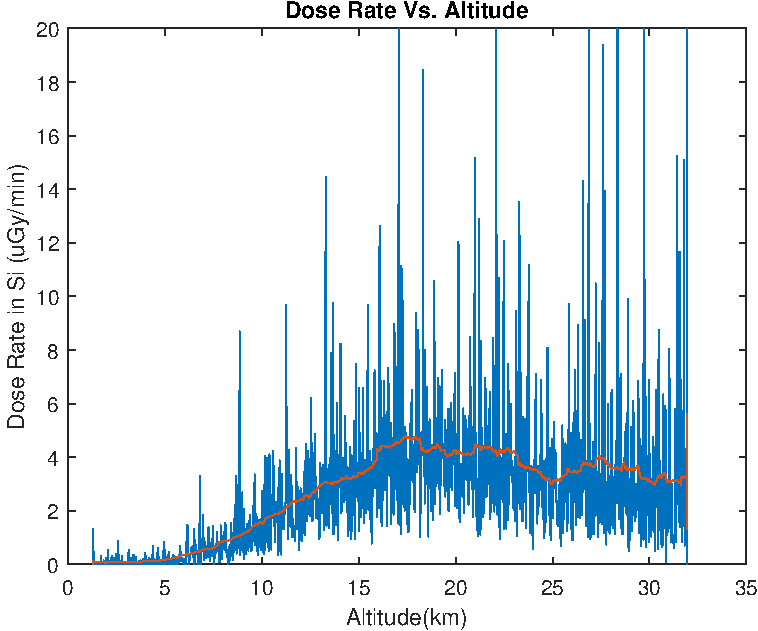
\includegraphics[scale=.5]{dva-cropped.pdf}
  \caption{Dose rate in silicon vs. altitude.}
  \label{fig:sub1}
\end{subfigure}%
\begin{subfigure}{.5\textwidth}
  \centering
  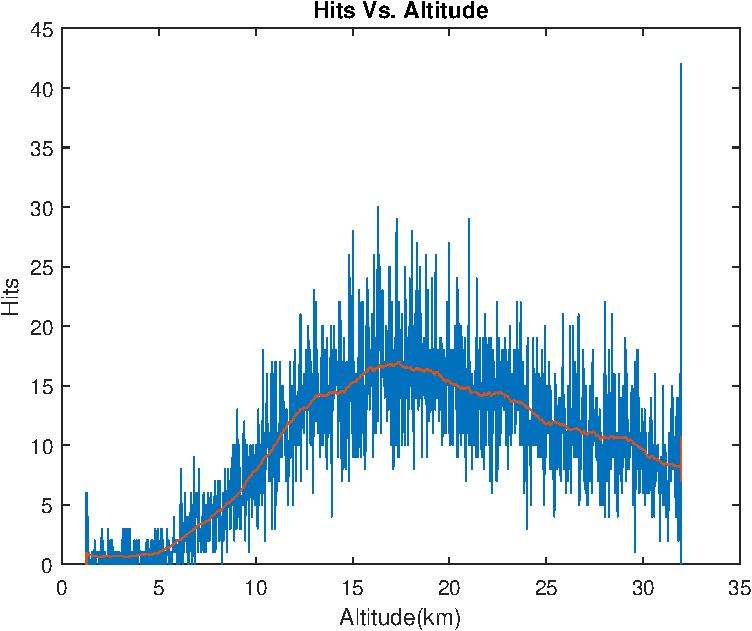
\includegraphics[scale=.5]{hva-cropped.pdf}
  \caption{Detector Hits vs. altitude.}
  \label{fig:sub2}
\end{subfigure}
\caption{Not sure what to put here yet.}
\label{fig:test}
\end{figure}

\begin{figure}[h]
\centering
\caption{Cluster Type Counts vs. altitude.}
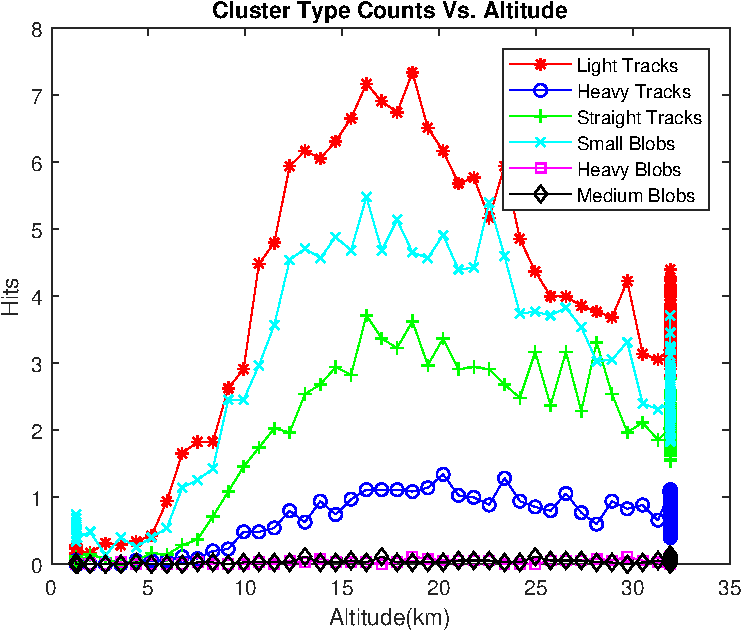
\includegraphics[scale=.5
]{ctva-cropped.pdf}
\end{figure}

\section{Discussion}
\label{Discussion}
\subsection{System Performance}
\subsection{Results}
% Discuss dose and particle count measurements as they relate to classical theory
\section{Conclusion}
\label{Conclusion}
% Overall, the device performed adequately and is potentially suitable for future applications in other areas
% Discuss future applications of the MiniPIX for compact, cheap and accurate(?) dosimeters on commercial airline flights

\section{Acknowledgements}
\label{Acknowledgements}
This will be a list populated by all the people that helped contribute to the project at one point or the other.  This includes those that helped us build briefly during the summer, and also those that helped review our paper.

\section{Funding Sources}
\label{funding}
STEM Center (need official title and name)

%% The Appendices part is started with the command \appendix;
%% appendix sections are then done as normal sections
%% \appendix

%% \section{}
%% \label{}

%% References
%%
%% Following citation commands can be used in the body text:
%% Usage of \cite is as follows:
%%   \cite{key}          ==>>  [#]
%%   \cite[chap. 2]{key} ==>>  [#, chap. 2]
%%   \citet{key}         ==>>  Author [#]

%% References with bibTeX database:
%%%%%%%%
%%%%%%%%\bibliographystyle{model1-num-names}
%%%%%%%%\bibliography{sample.bib}

%% Authors are advised to submit their bibtex database files. They are
%% requested to list a bibtex style file in the manuscript if they do
%% not want to use model1-num-names.bst.

%% References without bibTeX database:

\begin{thebibliography}{00}

%% \bibitem must have the following form:
%%   \bibitem{key}...
%%

%\bibitem{SORA}S.A. Garcia Morelos, F.Brooks, S.Oliver, A.Walker, K.D. Portillo, R.B. Masek, D.Mroczek, D.Pena, J.Juarez, A.Cruz, D. Henandez, S.George, D. Pattison, A.L.Renshaw. \textit{Scientific Report for the UH Team.} SORA 2017 Mission Webpage. \textit{http://laspace.lsu.edu/hasp/groups/Payload.php?py=2017&pn=10}.

\bibitem{minipix}MiniPIX - Miniaturized Portable USB Photon Counting Camera. (n.d.). Retrieved February 02, 2017, from \textit{http://advacam.com/camera/minipix}.

\bibitem{timepixiss} Stoffle, N., Pinsky, L. et al. Timepix-based radiation environment monitor mea-
surements aboard the International Space Station. Nucl. Instrum. Methods Phys.
Res., A, 782 (2015):143.

\bibitem{aircrewexposure} B.J. Lewis, M.J. McCall, A.R. Green, L.G.I. Bennett, M. Pierre, U.J. Schrewe, K. O'Brien, E. Felsberger; Aircrew Exposure from Cosmic Radiation on Commercial Airline Routes, Radiation Protection Dosimetry, Volume 93, Issue 4, 1 February 2001, Pages 293–314, \url{https://doi-org.ezproxy.lib.uh.edu/10.1093/oxfordjournals.rpd.a006442}
\bibitem{timepixdosimetry} Carlos Granja, Stanislav Pospisil,
Quantum dosimetry and online visualization of X-ray and charged particle radiation in commercial aircraft at operational flight altitudes with the pixel detector Timepix,
Advances in Space Research,
Volume 54, Issue 2,
2014,
Pages 241-251,
ISSN 0273-1177,
https://doi.org/10.1016/j.asr.2014.04.006.
(http://www.sciencedirect.com/science/article/pii/S0273117714002208)
Keywords: Radiation detection; Radiation exposure at aviation altitudes; Dose equivalent rate; Semiconductor pixel detector; Quantum dosimetry

%\bibitem{LSU}
%  Christner, B., Alleman, M., Bryan, N., Burke, S., Guzik, T.G., Granger, D., King, G. (2013) \textit{LSU HASP2013 PDF. Baton Rouge: Louisiana Space Consortium}.
%
%%\bibitem{SolidWorks}
%%  SolidWorks 3D CAD software \url{http://www.solidworks.com/}.
%
%\bibitem{Extremophiles}
%  Extremophiles \href{http://www.nytimes.com/2013/02/07/science/living-bacteria-found-deep-under-antarctic-ice-scientists-say.html}{http://www.nytimes.com/2013/02/07/science/living-bacteria-found-deep-\\under-antarctic-ice-scientists-say.html}.
%
%\bibitem{canales}
% Canales D. C. and Ehteshami A., \textit{An attempt to sample atmospheric bacteria}, Houston, TX, 2015, January 11.
%
%\bibitem{bexus}
%Urbar, J., Scheirich, J., Jakubek, J., 2011. Medipix/Timepix cosmic ray tracking on BEXUS stratospheric balloonflights. Nucl. Instrum. Methods A 633, S206-209.
%	
%%\bibitem{uv_irradiance}
%%  Calculating the UV Index. (2016, October 14). Retrieved June 03, 2017, from \url{https://www.epa.gov/sunsafety/calculating-uv-index-0}.
%
%%\bibitem{cleanbox}
%% Clean box material \url{https://www.mcmaster.com/\#uhmw-polyethylene/=1aijn1p}.
%
%\bibitem{valve}
% Valve data sheet \url{http://www.generant.com/Literature/Series\%20VRV\%20Product\%20Literature.pdf}.
%
\bibitem{advacam}
  ADVACAM at \url{http://www.advacam.com}
%
%\bibitem{medipix}
%  Medipix collaboration at \url{https://medipix.web.cern.ch/}.
%  
%\bibitem{stuartthesis} 22
%  George, S., \textit{Dosimetric Applications of Hybrid Pixel Detectors}, University of Wollongong, Australia, 2015.
%
%%\bibitem{mpdatasheet}
%%  ADVACAM, \textit{MINIPIX Version 1.0 Datasheet}, Retrieved from \url{http://www.widepix.cz/files/datasheets/MiniPIX\%20v1.0\%20Datasheet.pdf}.
%
%%\bibitem{mpjakubek}
%%  Jan Jakubek, \textit{Precise energy calibration of pixel detector working in time-over-threshold mode} Institute of Experimental and Applied Physics, Czech Technical University in Prague, Czech Republic, 2011.
%  
%
%    
%
%
%%\bibitem{magnetictool}
%%  United States National Oceanic and Atmospheric Administration, \textit{Magnetic Field Calculators} [Data sets], Retrieved from \url{https://www.ngdc.noaa.gov/geomag-web/#igrfwmm}.
%
%%\bibitem{gorman}
%%	Gorman, J. (2013, February 06). \textit{Scientists Find Life in the Cold and Dark Under Antarctic Ice.} Retrieved September 15, 2016, from Scientists Find Life in the Cold and Dark Under Antarctic Ice.
%	
% 
% 
%%\bibitem{pumpsource}
%%  \url{http://www.knfusa.com/?type=5600&amp;file=2079}.
%
%
%%\bibitem{Horneck}
%%  Horneck, G. 1993. The Biostack concept and its application in space and at accelerators: studies in Bacillus subtilis spores, p. 99-115. In C. E. Swenberg, G. Horneck, and E. G. Stassinopoulos (ed.), \textit{Biological effects and physics of solar and galactic cosmic radiation}[PDF], part A. Plenum Press, New York, NY. accessed 10/24/16  
%
%%\bibitem{Horneck} 
%%  Horneck, G. 2007. \textit{Space radiation biology}[PDF], p. 243-273. In E. Brinckmann (ed.), Biology in space and life on Earth. Wiley-VCH, Weinheim, Germany. Accessed 10/26/16
%
%%\bibitem{Horneck}
%%  Horneck, G., C. Baumstark-Khan, and G. Reitz. 2002. \textit{ Space microbiology: effects of ionizing radiation on microorganisms in space}[PDF], p. 2988-2996. In G. Bitton (ed.), The encyclopedia of environmental microbiology. John Wiley \& Sons, New York, NY. Accessed 10/30/16
%
%%\bibitem{Horneck}
%%  Horneck, G., C. Baumstark-Khan, and R. Facius. 2006. \textit{Radiation biology}[PDF], p. 292-335. In G. Cl?ment and K. Slenzka (ed.), Fundamentals of space biology. Kluwer Academic Publishers/Springer, Dordrecht, The Netherlands. accessed 11/4/16
%
%%\bibitem{Kiefer}
%%Kiefer, J., K. Schenk-Meuser, and M. Kost. 1996. \textit{Radiation biology}[PDF], p. 300-367. In D. Moore, P. Bie, and H. Oser (ed.), Biological and medical research in space. Springer, Berlin, Germany. accessed 11/9/16
% 
%	
%
%\bibitem{SamURD}
%	Alfonso Garcia Morelos, S. (2016, October 13).
%	\textit{A Novel Microbe Trap.}
%	Presentation at UH Undergraduate Research Day. \url{http://www.uh.edu/honors/undergraduate-research/}
%	
%	
%%\bibitem{StevenURD}
%
%%\bibitem{FreEttaWomensConference}
%
%%\bibitem{StevenSchoolPres}
%
%%\bibitem{StevenURD}
%%  Oliver, S. J. (2017, October 12). 
%%  \textit{Stratospheric Organism and Radiation Analyzer}
%%  Presentation at UH Undergraduate Research Day. Retrieved October 12, 2017, from \url{http://www.uh.edu/honors/undergraduate-research/events/urday2017/}
%
%%\bibitem{StevenSchoolPres}
%%  Oliver, S. J. (2017, November 4). 
%%  \textit{STEM Life at UH}
%%  Presentation at UH Gathering of the Eagles STEM Symposium. \url{https://www.uh.edu/news-events/stories/2016/November/110416EaglesSTEM.php}
%
%%\bibitem{Fre}
%%  Brooks, F. (2017, January 14).
%%  \textit{Stratospheric Organism and Radiation Analyzer}
%%  Presentation at Rice University, APS Conferences for Undergraduate Women in Physics (CUiP). \url{http://www.google.com/url?q=http%3A%2F%2Fwww.aps.org%2Fprograms%2Fwomen%2Fworkshops%2Fcuwip.cfm&sa=D&sntz=1&usg=AFQjCNE5pImV-SVrb87CvgAa9RSfeCrYXg}  
%  
%%\bibitem{SamAPS}
%%	Alfonso Garcia Morelos, S. (2017, October 20).
%%	\textit{Stratospheric Organism and Radiation Analyzer}
%%	Retrieved October 20, 2017, from \textit{Bulletin of the American Physical Society}. \url{https://meetings.aps.org/Meeting/TSF17/Session/E5.3}
%	
%  
%%  \bibitem{MIT}
%%	MIT-Lemelson Award 2018.
%%	\url{https://lemelson.mit.edu/}

\end{thebibliography}


\end{document}

%%
%% End of file `elsarticle-template-1-num.tex'.
              
\grid
\grid
\grid
